%!TEX TS-program = xelatex
%!TEX encoding = UTF-8 Unicode

% Load Thesis Class
\documentclass{DEIThesis}

% Development and testing of the 3302-2033 IEEE standard-compliant software for a high quality audio codec for Musical Cultural Heritage preservation using Test-Driven Development approach
\title{Sviluppo e testing di Software conforme allo standard IEEE 3302-2022 per una codifica audio ad alta qualità per la conservazione del patrimonio culturale musicale utilizzando un approccio Test-Driven Development}

\author{Alberto Pasqualetto}
\studentId{2000162}

% Advisor
\advisor{Prof. Sergio Canazza}

% If you are co-advised
\coadvisor{}
\coadvisorsUniversity{}

\university{University of Padova}
\bachelorname{Computer Engineering}
\academicYear{2022/2023}

\begin{filecontents*}[overwrite]{\jobname.xmpdata}
    \Title{Sviluppo e testing di Software conforme allo standard IEEE 3302-2022 per una codifica audio ad alta qualità per la conservazione del patrimonio culturale musicale utilizzando un approccio Test-Driven Development}
    \Author{Alberto Pasqualetto}
    \Language{it-IT}
    \Keywords{Computer Engineering \sep Audio Preservation \sep MPAI \sep Test Driven Development \sep Software Testing}
\end{filecontents*}

% Document

\begin{document}
    % The front matter (Cover, ToC, Abstract, etc...)
    \frontmatter

    % The main content
    \mainmatter
    
    %!TEX root = ../main.tex

\chapter{Digitalizzazione di audio analogico} \label{chp:digitalizzazione}

Preservare dall'oblio il proprio patrimonio culturale è sicuramente una delle necessità più antiche dell'uomo.

Al contrario della conservazione passiva, che consiste nella sola salvaguardia dei documenti nella loro dimensione fisica; l'unica soluzione per preservare a lungo termine il materiale analogico è la digitalizzazione, ovvero una conservazione di tipo attivo.
Tra il materiale da digitalizzare, quello audio-visivo è sicuramente uno dei più complicati per via della necessità di preservare sia il suo stato e la sua performance attuali, seppur il documento sia rovinato dal tempo o dall'usura, compreso di tutte le informazioni accessorie, sia di disporre di una copia cosiddetta "di accesso" in maniera tale da essere riprodotta agilmente con tecnologie odierne.

Molte organizzazioni quali archivi, librerie e musei non hanno ancora messo in pratica misure atte a preservare a tempo indeterminato il loro patrimonio culturale e ciò si verifica non solo nelle nazioni a più basso sviluppo umano come quelle dell'Africa subsahariana \cite{rakemaneChallengesManagingPreserving2021}, ma anche in nazioni a più alto indice di sviluppo umano come l'Italia \cite{raimoDigitalizationCulturalIndustry2022} presentando criticità non del tutto dissimili come, per esempio, la mancanza di fondi per via della poca importanza riposta nella causa. % anche loro hanno trovato l'istituzione ed implementazione di politiche di conservazione come soluzione

I musei che negli anni e soprattutto con l'avvento del COVID-19 si sono dovuti adeguare introducendo la tecnologia digitale dapprima nelle loro strutture per migliorare l'esperienza dei visitatori e poi in rete creando delle mostre virtuali generando anche maggiori visite ed incassi \cite{raimoDigitalizationCulturalIndustry2022}, ora possono sfruttare la digitalizzazione con lo scopo accessorio di creare nuove esperienze online.
Questo sforzo è anche in linea con le raccomandazioni dell'UNESCO \cite{unescoRecommendationConcerningProtection} in riferimento all'importanza della tecnologia in ambito educativo e culturale.


% TODO mostrare meglio la differenziazione tra audio e generico
\section{Filologia e Fedeltà} \label{sec:filologia-fedeltà}
La maniera più basilare di procedere alla digitalizzazione è registrare soltanto l'informazione primaria ovvero, nel caso di un prodotto sonoro, il segnale audio.
Per digitalizzare, invece, il prodotto in maniera filologicamente corretta è necessario memorizzare anche le informazioni ausiliarie come le annotazioni sul contenitore o sul supporto, i rumori presenti sul sistema di registrazione originale, le alterazioni fisiche del supporto, il marchio e modello del supporto ed altri metadati, oltre alla storia del tramandamento del documento (archiviazione, duplicazione, ecc.) \cite[p. 59]{prettoComputingMethodologiesSupporting2018}.

Per ottenere il massimo livello di aderenza alla realtà: la fedeltà, si deve assicurare, oltre che una riproduzione audio fedele, anche una simulazione dell'esperienza di interazione col dispositivo di riproduzione ed una riproduzione dei metadati e delle informazioni contestuali come ad esempio mostrato nel capitolo 3 di \textcite{fantozziTapeMusicArchives2017}.

In certi casi può essere utile operare delle modifiche alla traccia digitalizzata o ad una sua copia nel caso in cui ci siano degli errori o delle corruzioni nel supporto originario o nella digitalizzazione. Tali modifiche possono essere correttive atte a ripristinare la corretta riproduzione secondo i canoni dettati dalla filologia, oppure possono essere utili a creare una copia di accesso a discapito della fedeltà assoluta.


\section{Digitalizzazione manuale e automatizzazione} \label{sec:digitalizzazione-man-vs-auto}
Il trasferimento da analogico a digitale dipende ancora dall'esperienza dell'operatore (dalle sue valutazioni e scelte se intervenire o meno), ciò può comportare l'introduzione di errori indesiderati causati dalla perdita di attenzione umana in seguito a numerose ore di lavoro con riflessi negativi sul valore dei documenti creati e sull'affidabilità dell'intera collezione.
Per questo motivo è importante l'automatizzazione delle attività ripetitive in modo da minimizzare tali errori, ma anche da tagliare i costi e risparmiare tempo di lavoro \cites[cap. 2.1]{fantozziTapeMusicArchives2017}[es. 5]{mpaiApplicationNoteRev}.


\section{Il Centro di Sonologia Computazionale ed il suo metodo di digitalizzazione} \label{sec:csc-digitalizzazione}
Il \ac{CSC} del \ac{DEI} dell'Università di Padova, che da circa 50 anni opera nella ricerca in ambito acustico \cite{canazzaGestureMusicComputer2022}, è uno dei poli più all'avanguardia per quanto concerne la digitalizzazione di supporti musicali, nello specifico di nastri magnetici a bobina aperta (open reel tape) ed è uno dei maggiori sostenitori dell'utilizzo di automazioni nel processo di trasporto da analogico a digitale.

Dato che documentare il processo che ha generato la copia di conservazione è importante nel campo dell'audio, visto che il supporto originario potrebbe diventare irrecuperabile in futuro, il \ac{CSC} negli anni, collaborando con diversi archivi digitali, si è impegnato a sviluppare una tecnica di digitalizzazione "filologicamente informata" e di documentare la procedura in maniera accurata, verificabile ed oggettiva con l'obiettivo di creare uno standard.

L'innovazione principale in questo protocollo è la registrazione video del nastro magnetico contemporaneamente alla registrazione della traccia audio: viene effettuata la ripresa ai fini di catturare le immagini del nastro in corrispondenza della testina di registrazione ed in corrispondenza del capstan, le regioni interessate si possono trovare in figura \ref{fig:tape-areas}.

\begin{figure}[h]
    \centering
    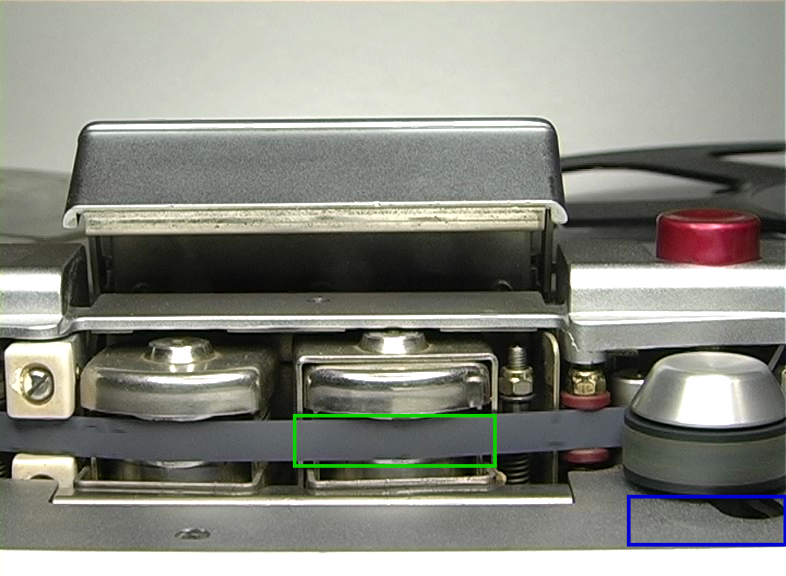
\includegraphics[width=\textwidth]{tape_areas.png}
    \caption{Regioni di interesse sotto alla testina di registrazione ed al capstan \cite{russoEnhancingPreservationRestoration}}
    \label{fig:tape-areas}
\end{figure}

La porzione vicina al capstan\footnote{Riquadro blu in figura \ref{fig:tape-areas}} serve ad individuare l'inizio della registrazione in quanto esso trasla verso il nastro nel momento in cui il motore viene azionato; mentre la sezione davanti alla testina di registrazione\footnote{Riquadro verde in figura \ref{fig:tape-areas}} serve ad individuare, tramite tecniche di intelligenza artificiale, tutte le alterazioni del retro nel nastro che, da ora in poi, chiameremo "irregolarità"; alcuni esempi sono giunzioni, scritte e parti visivamente danneggiate o rovinate, vedi figura \ref{fig:nastro-irrs}.
Questi sono parte dei metadati citati all'inizio di questa sezione.
L'utilità di raccogliere tali dati legati alla traccia audio è quella, oltre che di catturare il documento nella sua essenza più completa, anche di poter ricollegare la performance di una qualsiasi porzione della traccia audio ad un'eventuale irregolarità sul nastro ed eventualmente agire di conseguenza.

\begin{figure}
     \centering
     \begin{subfigure}{0.45\textwidth}
         \centering
         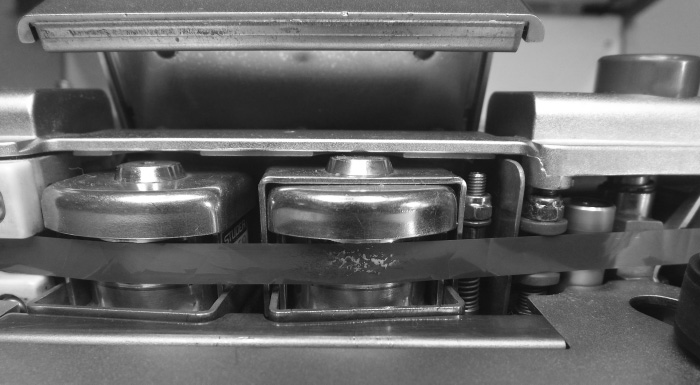
\includegraphics[width=\textwidth]{nastro_rovinato.png}
         \caption{Porzione di nastro rovinata \cite{prettoComputingMethodologiesSupporting2018}}
         \label{fig:nastro-rovinato}
     \end{subfigure}
     \hfill
     \begin{subfigure}{0.45\textwidth}
         \centering
         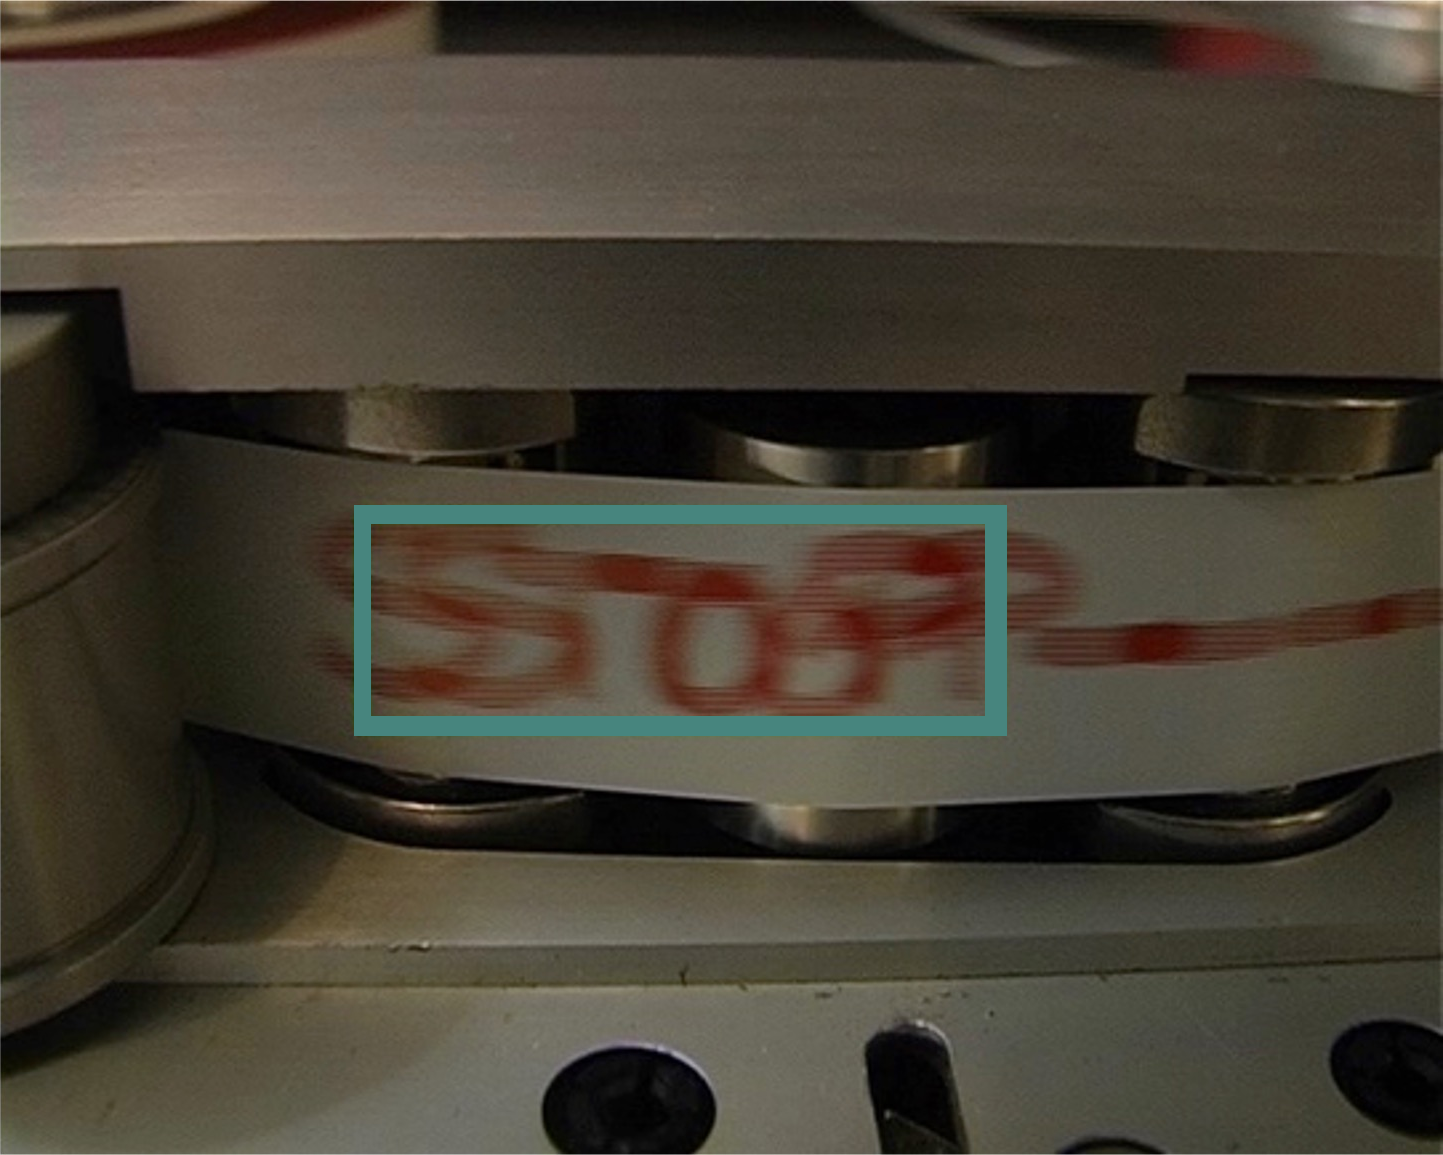
\includegraphics[width=\textwidth]{nastro_testo.png}
         \caption{Testo su nastro \cite{canazzaGestureMusicComputer2022}}
         \label{fig:nastro-testo}
     \end{subfigure}
        \caption{Alcuni esempi di irregolarità}
        \label{fig:nastro-irrs}
\end{figure}

La procedura creata dal \ac{CSC} prevede anche una gestione di tracce audio catturate a velocità o equalizzazione incorrette:

La velocità, misurata in pollici per secondo (\textit{inches per second}, ips in inglese), è solitamente impostata a sottomultipli binari di \qty{30}{ips} e viene regolata in base alla qualità di registrazione ed alla durata di un nastro che l'artista ha voluto ottenere, in generale maggiore è la velocità, maggiore sarà la qualità di registrazione e minore la durata del nastro.
Può accadere che nello stesso nastro digitalizzato siano presenti tracce a velocità diverse ed alcuni motivi potrebbero essere le aggiunte di altro nastro, registrato diversamente, per eseguire del montaggio, oppure la diminuzione di velocità all'avvicinarsi della fine del nastro in maniera tale da concludere la performance senza dover utilizzare un nuovo supporto, oppure ancora la registrazione di più performance scorrelate tra loro all'interno stesso nastro.

Per quanto riguarda l'equalizzazione invece, le curve di equalizzazione\footnote{L'equalizzazione è una tecnica di filtraggio che permette di variare l'ampiezza delle frequenze di un segnale audio; una curva di equalizzazione è ottenuta dalla combinazione dei risultati delle due curve $N(DB)=10 \log(1 + \frac{1}{4 \pi^2 f^2 t_2^2}) - 10 \log(1+4\pi^2 f^2 t_1^2)$ dove $f$ è la frequenza in \unit{\Hz} e $t_1$ e $t_2$ sono costanti di tempo in secondi.} solitamente sono quelle dettate dagli standard \acs{CCIR}, utilizzato in Europa, e \acs{NAB}, utilizzato in USA.

Il CSC utilizza ancora una volta un modello di machine learning allenato a riconoscere in porzioni di audio di \qty{500}{\ms} se la velocità e la curva di equalizzazione impostate al momento del trasferimento da analogico a digitale sono corrette ed a classificarle con le velocità ed equalizzazione corrette; per fare ciò si da in pasto al modello pre-allenato il rumore estrapolato dai silenzi presenti nell'interezza della traccia audio ed i relativi primi 13 coefficienti spettrali mel (\acfi{MFCC}\footnote{I coefficienti spettrali mel sono una rappresentazione del segnale acustico, solitamente sono utilizzati per rappresentare le caratteristiche generali del segnale acustico e vengono spesso utilizzati in applicazioni di riconoscimento del parlato e recupero di informazioni musicali; sono calcolati a partire dal segnale audio su cui viene applicata la trasformata di Fourier con cui si calcola la potenza dello spettro e la si riscala con la scala mel (una scala basata sulla percezione dell'altezza del suono), dopodiché vengono applicati il logaritmo e la trasformata discreta del coseno; i coefficienti sono le ampiezze dello spettro risultante.}).
% TODO scrivere successo 93,7% di aa?

    %!TEX root = ../main.tex

\chapter{MPAI} \label{chp:mpai}
Dalle ceneri del rinomato \ac{MPEG}, nel luglio 2020 nasce \ac{MPAI}\footnote{\url{https://mpai.community}}.

\ac{MPAI} è un'organizzazione non profit che, ancora guidata da Leonardo Chiariglione, ha come obiettivo la promozione dell'uso efficiente dei dati\footnote{Per dati \ac{MPAI} intende, per esempio, dati mediatici, manifatturieri, automobilistici, sanitari e generici. \cite{mpaiMPAICommunity}.} tramite lo sviluppo di specifiche tecniche per la codifica di qualunque tipo di dato facendo uso dell'intelligenza artificiale e la semplificazione dell'utilizzo di tali codifiche imponendo ai detentori di proprietà intellettuale di stabilire delle licenze per framework (\acs{AIF}), invece di dover essere legati ai brevetti e creare delle \textit{patent pool} \cite{mpaiMPAICommunity}. Sostanzialmente l'organizzazione si pone come missione quella di porre ordine nel mondo delle codifiche utilizzanti l'IA e di farlo semplificando il metodo di accesso alle proprie tecnologie rispetto ad \ac{MPEG}.
\ac{MPAI} opera attraverso la collaborazione delle varie parti interessate, tra cui l'università di Padova tramite il suo spin-off \href{www.audioinnova.com}{Audio Innova}.

In questi tempi l'utilizzo dell'intelligenza artificiale sta crescendo in maniera esponenziale e si sta avvicinando all'utente comune tramite la miriade di piattaforme online che sono nate, un esempio è \href{https://chat.openai.com}{ChatGPT} che ha raggiunto quota 100 milioni di utenti attivi in soli 2 mesi, raggiungendo il primato di applicazione ad uso privato con la crescita più veloce della storia.\footnote{\url{https://www.reuters.com/technology/chatgpt-sets-record-fastest-growing-user-base-analyst-note-2023-02-01/}} Nonostante il suo, come visto, uso spropositato l'IA è di fatto una tecnologia difficilmente comprensibile dalle masse; ciò porta l'utente a non capire che il \textit{chatbot} con cui sta interagendo, non replichi utilizzando un principio di causalità, ma piuttosto segua dei pattern linguistici i quali non sempre portano a risposte corrette, nonostante l'autorevolezza col quale l'IA sembri scrivere.

Il comitato di \ac{MPAI} si impegna ad affrontare col coinvolgimento di esperti esterni gli emergenti quesiti etici, i quali sono molto rilevanti a causa del rapido e soltanto recente sviluppo dell'IA.

Il progetto comprende diverse aree d'effetto tra cui il dialogo uomo-macchina, l'esperienza audio, la compressione video, l'esperienza di gioco online, la creazione di esperienze collaborative nel metaverso, la codifica di dati sanitari, i veicoli a guida autonoma e molti altri e la lista è in continua espansione.\footnote{Tutti i vari progetti sono visualizzabili sul \href{https://mpai.community/standards/}{sito di \ac{MPAI} alla voce \textit{Standards}}.}


\section{MPAI-AIF, \acs{AIW} e \acsp{AIM}} \label{sec:aif-aiw-aim}
Ogni standard \ac{MPAI} è un \ac{AIF} \cite{mpaiMPAIAIFMPAICommunity}: un ambiente che comprende diversi \ac{AIW}, ognuno che descrive un certo caso d'uso. I blocchi costituenti un workflow sono detti \acp{AIM} ed ogni modulo è definito dalla sintassi e dalla semantica delle proprie interfacce di input e output, l'implementazione (hardware o software che sia) non è specificata; i vari moduli svolgono delle specifiche attività e sono interconnessi a formare un AIW come si può vedere dalla figura \ref{fig:mpai-aif-architecture}.

\acs{AIF}, il modello fondante gli altri standard dell'organizzazione è stato adottato dall'\ac{IEEE} col nome \textit{IEEE 3301-2022} \cite{ieeeStandard3301-2022}.

\begin{figure}[h]
    \centering
    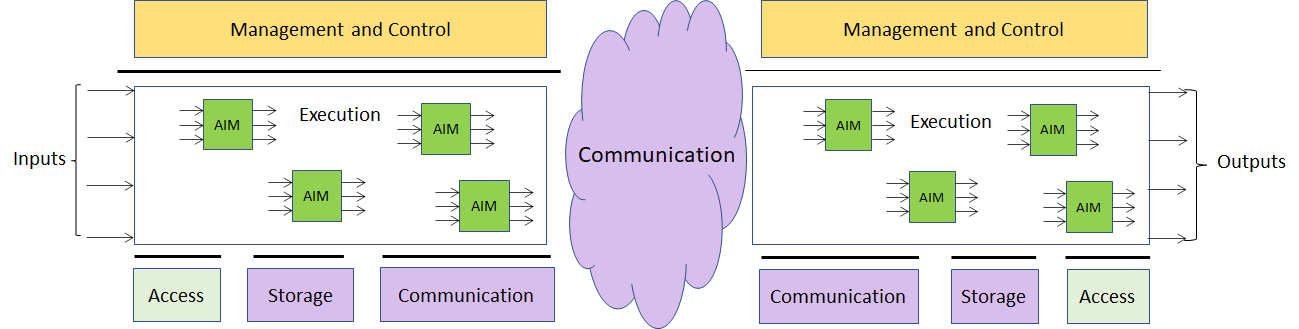
\includegraphics[width=\textwidth]{mpai-aif-architecture.png}
    \caption{Architettura di \acs{AIF} \cite{leonardoBlogNewWayDevelop2020}}
    \label{fig:mpai-aif-architecture}
\end{figure}


\section{Struttura di uno standard MPAI} \label{sec:standard-mpai} % e come implementarlo
Lo sviluppo di uno standard MPAI segue le fasi mostrate in figura \ref{fig:mpai-standard-stages}.    % TODO scrivere di più?

\begin{figure}[h]
    \centering
    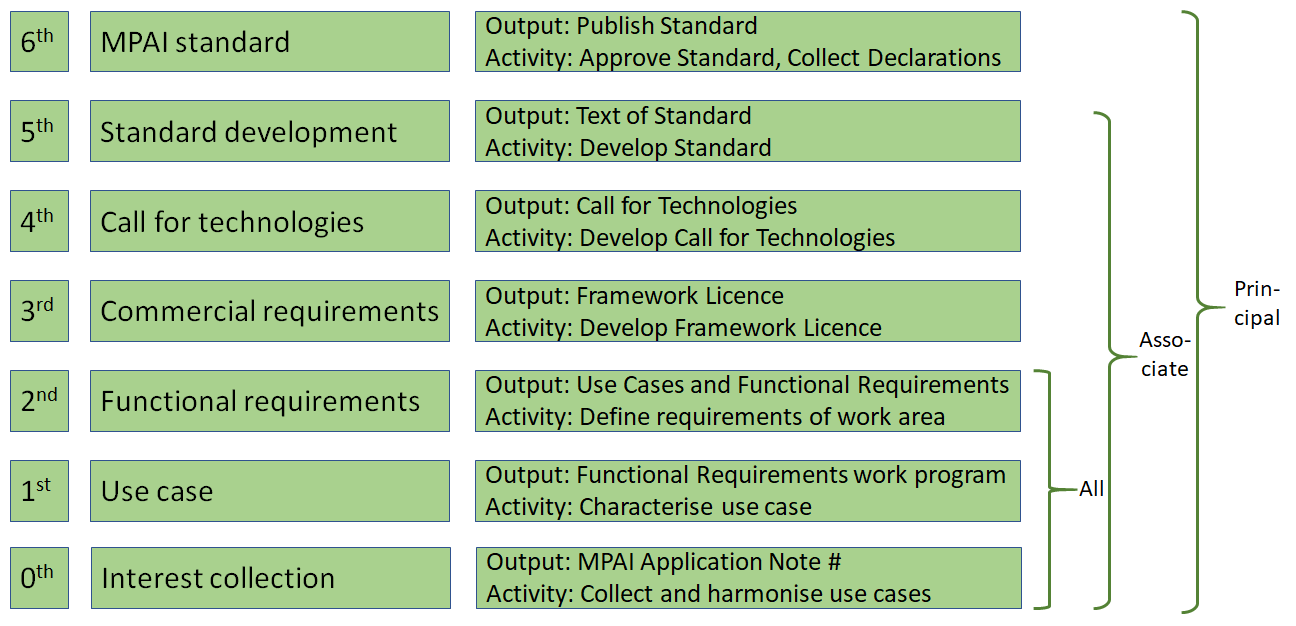
\includegraphics[width=\textwidth]{mpai-standard-stages.png}
    \caption{Le fasi dello sviluppo di uno standard \acs{MPAI} \cite{leonardoBlogNewWayDevelop2020}}
    \label{fig:mpai-standard-stages}
\end{figure}

Uno standard \ac{MPAI} è composto da un insieme di 4 documenti con i relativi software e dataset \cite{mpaiStructureMPAIStandards}:
\begin{description}
    \item[Specifiche tecniche (\textit{Technical Specification})] Contiene le norme che un'implementazione conforme deve necessariamente seguire; solitamente è un insieme di casi d'uso. Per ogni caso d'uso viene specificato l'\ac{AIW} che lo implementa con le funzioni che esegue, la sintassi e la semantica dei suoi dati in input ed output; la topologia degli \acp{AIM} costituenti l'\ac{AIW} e, per ogni \ac{AIM}, la loro funzione e la sintassi e la semantica dei loro input ed output. 
    \item[Software di riferimento (\textit{Reference Software})] Contiene il codice sorgente dell'implementazione delle specifiche tecniche dell'\ac{AIF} e dei suoi \ac{AIW} esponendo le interfacce dei propri \acp{AIM}. Inoltre il software deve essere fornito di un metodo per l'uso, la sua documentazione necessaria\footnote{Una \ac{KB}} ed eventualmente dei dati di esempio.
    \item[Test di conformità (\textit{Conformance Testing})] Un insieme di vincoli relativi all'output generato da un dato input a cui un'implementazione deve sottostare per essere definita conforme. Questo documento viene trattato in maniera più approfondita al capitolo \ref{chp:conformancetesting}.
    \item[Valutazione delle prestazioni (\textit{Performance Assessment})] Definisce gli attributi di Affidabilità (rispetto dello standard), Robustezza (capacità di gestione di nuovi dati), Equità (IA unbiased\footnote{Un'intelligenza artificiale può essere \textit{biased}, ovvero può "avere pregiudizi"; nel caso ottimo sono molto limitati (IA unbiased) perchè portano ad assunzioni errate.}) e Replicabilità (della valutazione) che vengono utilizzati per attribuire un voto all'implementazione (eventualmente dipendente da un certo dominio di applicazione).
\end{description}

\begin{adjustbox}{width=\textwidth}
    \begin{tikzpicture}[
        state/.style={rectangle, draw=black, align=center, minimum size=5mm},
    ]
        %Nodes
        \node[state]  (TS)                    {Specifiche\\tecniche};
        \node[state]  (RS)    [right=of TS]   {Software\\di riferimento};
        \node[state]  (CT)    [right=of RS]   {Test\\di conformità};
        \node[state]  (PA)    [right=of CT]   {Valutazione\\delle prestazioni};
        
        %Lines
        \draw[->] (TS.east) -- (RS.west);
        \draw[->] (RS.east) -- (CT.west);
        \draw[->] (CT.east) -- (PA.west);
    \end{tikzpicture}
\end{adjustbox} % TODO decidere se inserire in una figure?


\section{MPAI-CAE} \label{sec:mpai-cae}
Tra i vari standard/framework, \ac{CAE} si occupa di utilizzare le informazioni sul tipo di esperienza audio vissuta dall'utente (intrattenimento, teleconferenza, restauro, ...) e 'informazione del contesto in cui si trova (a casa, in auto, in mobilità, in studio, ...) per agire sul contenuto dell'audio in input e fornire i risultati desiderati \cite{mpaiMPAICAE}.

Sono considerati 4 casi d'uso:
\begin{description}
    \item[\ac{EES}] Permette all'utente di scegliere un'emozione ed ottenere successivamente una traccia audio di parlato con la tonalità specifica tipica dell'espressività indicata.
    \item[\ac{ARP}] Permette di creare copie di audio digitalizzato, valido per una conservazione a lungo termine e per una riproduzione corretta della registrazione.
    \item[\ac{SRS}] Permette di ripristinare un segmento danneggiato di traccia audio contenente il parlato di un singolo oratore sintetizzando la voce della parte corrotta.
    \item[\ac{EAE}] Permette di migliorare la qualità sonora in un'audioconferenza utilizzando i segnali registrati da array di microfoni rimuovendo rumori di fondo e artefatti acustici.
\end{description}

\ac{CAE} è stato adottato dall'\ac{IEEE} come standard \textit{IEEE 3302-2022} \cite{ieeeStandard3302-2022}.

Nel documento \citetitle{ieeeStandard3302-2022} si possono trovare tutte le informazioni sullo standard.


\subsection{MPAI-CAE-ARP} \label{ssec:mpai-cae-arp} % è l'implementazione del metodo del CSC, cos'è un codec, cosa fa, quali sono i suoi moduli
La procedura di digitalizzazione del \ac{CSC} introdotta nella sezione \ref{sec:csc-digitalizzazione} è stata proposta ad \ac{MPAI} ed è stata riconosciuta per la sua efficacia ed affidabilità, perciò è stata adottata come use case di \ac{CAE} col nome \acf{ARP}.\footnote{Le informazioni di questa sottosezione sono tratte da \cite{mpaiMPAIDataCoding}; maggiori informazioni nelle specifiche tecniche \cite{ieeeStandard3302-2022} e nella video presentazione del software di riferimento \cite{mpaistandardsMPAIPresentsContextbased2023}}

Il \ac{CSC}, con l'aiuto di vari collaboratori, ha prodotto anche un software di riferimento per \ac{ARP}, il quale non è altro che una codifica\footnote{Un codec (audio) è un software o un dispositivo che codifica o decodifica un segnale o uno stream di dati secondo una specifica convenzione.} audio lossless.

Nel 2023 Audio Innova è stata insignita del \textit{Cannes Neurons Award 2023 Palm d'Or} per il miglior progetto di utilizzo creativo di IA, \ac{ARP}, al World AI Cannes festival.\footnote{\url{https://mpai.community/2023/02/17/mpai-member-audio-innova-srl-received-the-cannes-neurons-award-2023-palm-dor/}}

Dati in input (vedi figura \ref{fig:arp-workflow}):
\begin{description}
    \item[Preservation Audio File] La copia digitalizzata dell'audio.
    \item[Preservation Audio-Visual File] Il file video prodotto dalla ripresa della testina di registrazione e del capstan (come in figura \ref{fig:tape-areas}).
\end{description}

Si ottengono in output (vedi figura \ref{fig:arp-workflow}):
\begin{description}
    \item[Access Copy Files] Il file audio restaurato, una lista delle modifiche effettuate, la lista delle irregolarità con relativa classificazione e le loro istantanee dal video.
    \item[Preservation Master Files] Il file audio di input, il file video con l'audio sostituito da quello registrato e sincronizzato, la lista delle irregolarità con relativa classificazione e le loro istantanee dal video.
\end{description}

\begin{figure}[H]
    \centering
    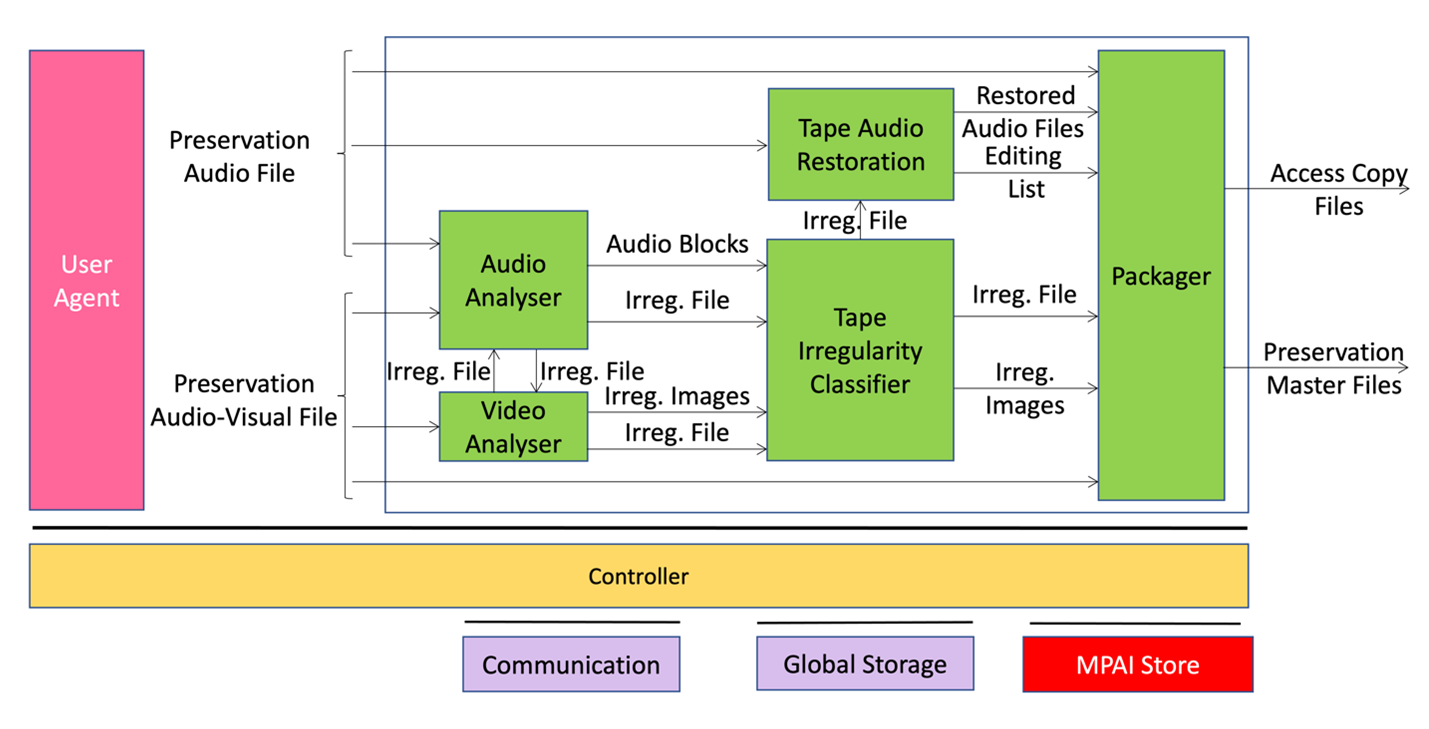
\includegraphics[width=\textwidth]{arp-workflow.png}
    \caption{\ac{AIW} di \acl{ARP}}
    \label{fig:arp-workflow}
\end{figure}

Facendo riferimento alla figura \ref{fig:arp-workflow} gli \acp{AIM} di \ac{ARP} sono:
\begin{description}
    \item[Audio Analyser] È l'\ac{AIM} che rileva le irregolarità nell'audio, estrae i segmenti di \qty{500}{\ms} in loro corrispondenza e li invia al classificatore.
    \item[Video Analyser] È l'\ac{AIM} che rileva le irregolarità nel video e cattura delle immagini in loro corrispondenza.
    \item[Tape Irregularity Classifier] È l'\ac{AIM} che classifica le irregolarità di audio e video a partire dalle irregolarità rilevate da audio analyser e video analyser.   % TODO nel codice è compreso in aa e va? -> chiedere
    \item[Tape Audio Restoration] È l'\ac{AIM} che corregge velocità, equalizzazione e registrazione a rovescio dell'audio.
    \item[Packager] È l'\ac{AIM} che produce Access Copy Files e Preservation Master Files a partire dai file ricevuti dall'output degli altri \acp{AIM}.
\end{description}

Si osserva nella letteratura afferente al \ac{CSC} che la classificazione dei problemi dalla traccia audio ha un'accuratezza del $93,7\%$ (esempio in figura \ref{fig:confusion-matrix-audio-classification}) \cite[min. 35:10]{mpaistandardsMPAIPresentsContextbased2023}, mentre per la classificazione dalle immagini si raggiungono valori $\geq 98,9\%$ (esempio in figura \ref{fig:confusion-matrix-audio-classification}) \cite[fig. 3 e p. 70]{prettoComputingMethodologiesSupporting2018}.

\begin{figure}[h]
    \begin{minipage}{\textwidth}
        \centering
        \begin{subfigure}{0.8\textwidth}
            \centering
            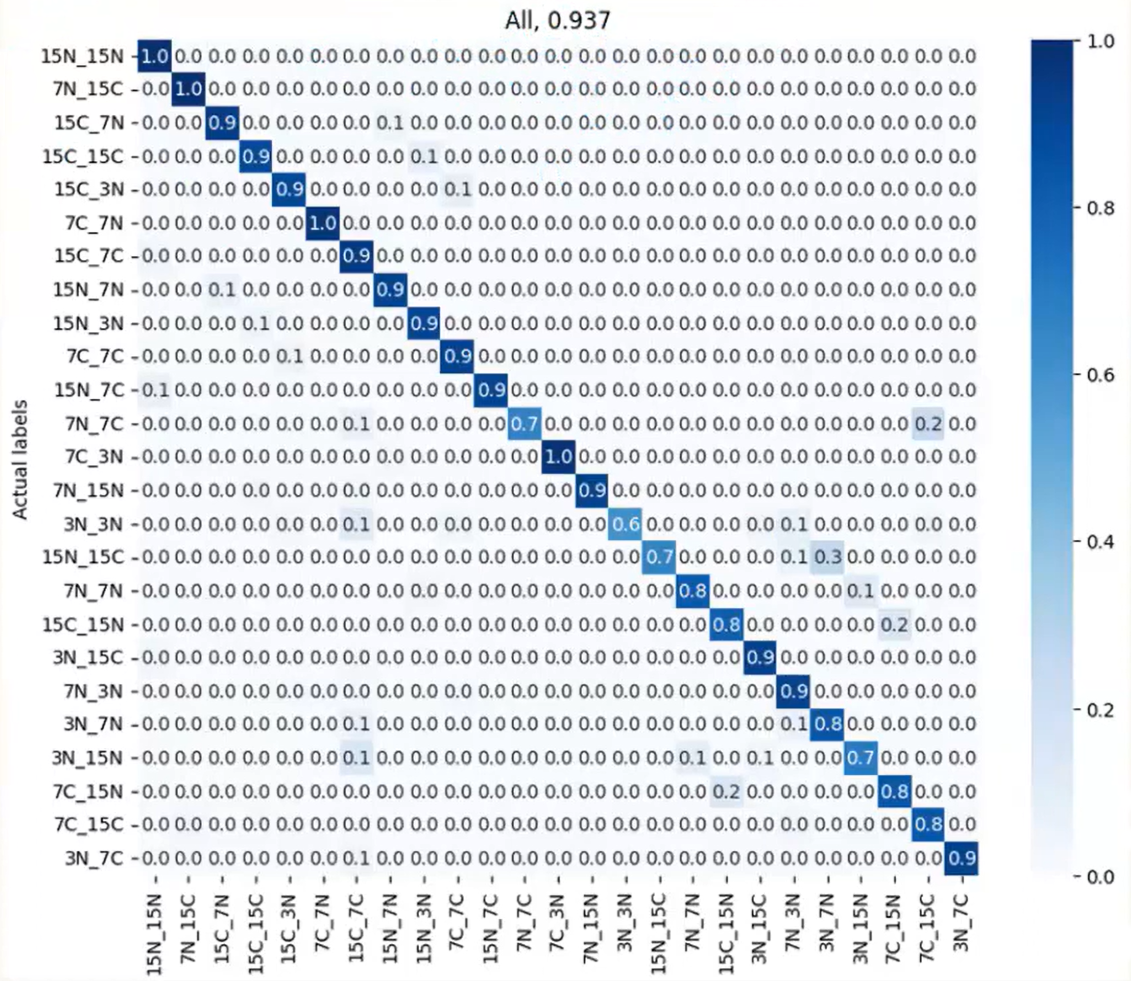
\includegraphics[width=\textwidth]{confusion-matrix-audio-classification.png}
            \caption{Matrice di confusione di classificatore audio \cite[min. 35:10]{mpaistandardsMPAIPresentsContextbased2023}}
            \label{fig:confusion-matrix-audio-classification}
        \end{subfigure}
        \par\bigskip
        \begin{subfigure}{0.9\textwidth}
            \centering
            \begin{subfigure}{0.45\textwidth}
                \centering
                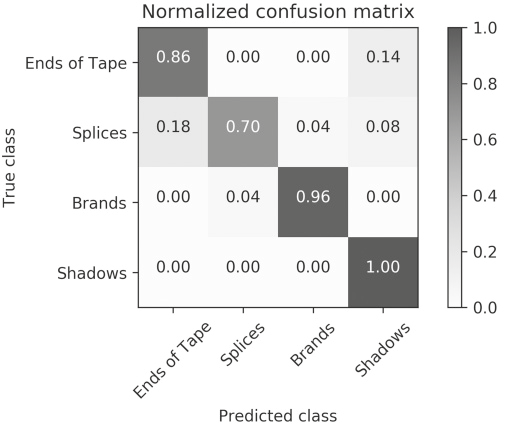
\includegraphics[width=\textwidth]{confusion-matrix-video-classification-7dot5ips-tape.png}
                \caption{Matrice di confusione di classificatore video, esperimento a velocità \qty{7,5}{ips}}
                \label{fig:confusion-matrix-video-classification-7dot5ips-tape}
            \end{subfigure}
            \hfill
            \begin{subfigure}{0.45\textwidth}
                \centering
                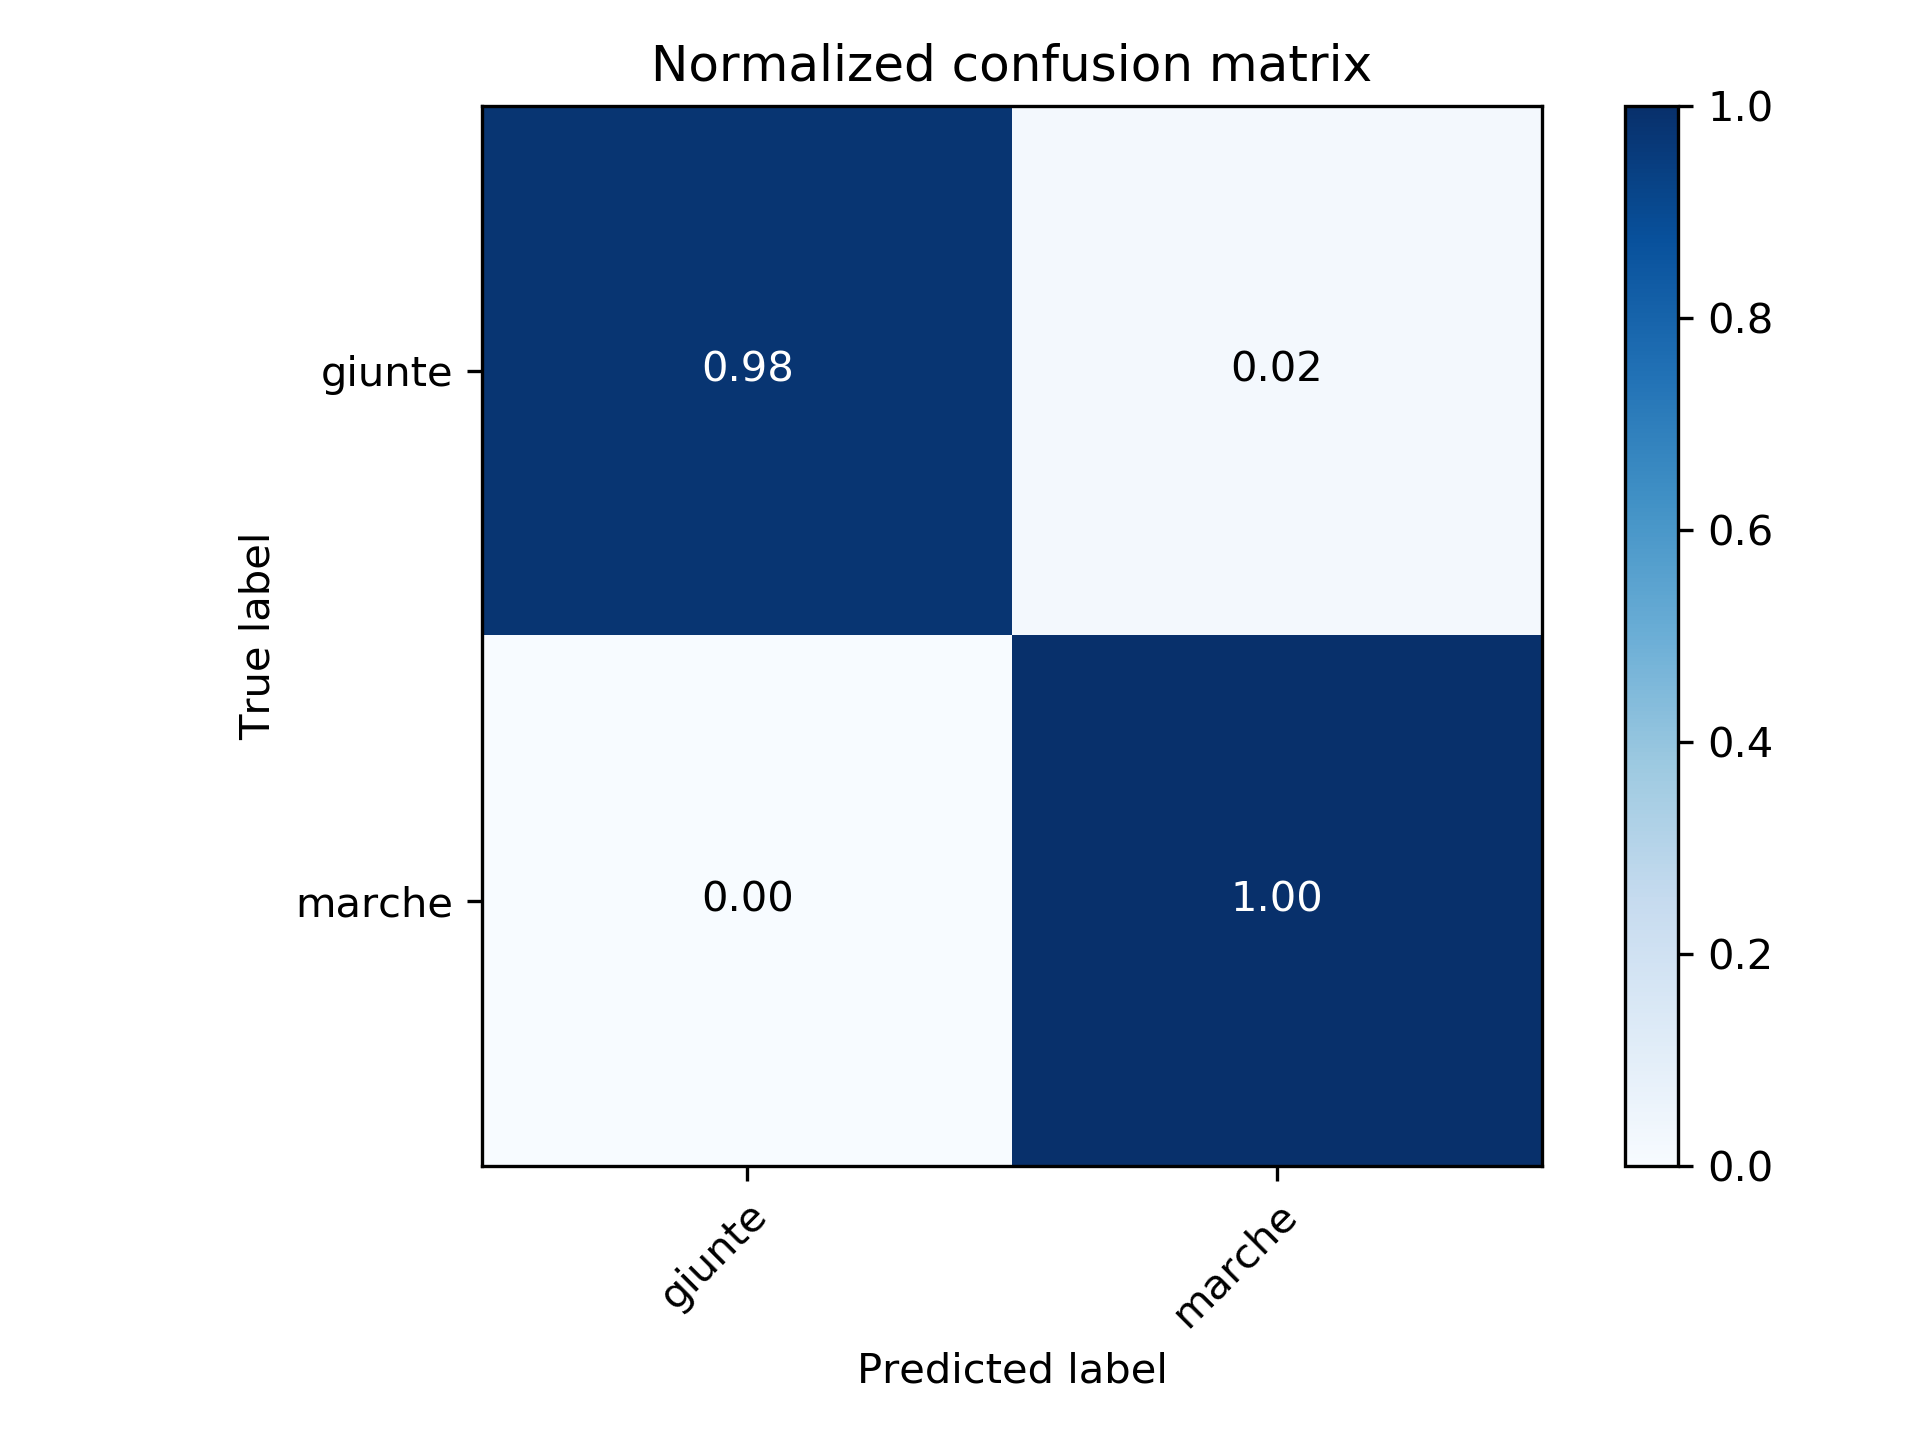
\includegraphics[width=\textwidth]{confusion-matrix-video-classification-15ips-tape.png}
                \caption{Matrice di confusione di classificatore video, esperimento a velocità \qty{15}{ips}}
                \label{fig:confusion-matrix-video-classification-15ips-tape}
            \end{subfigure}
            \caption{Matrice di confusione di classificatore video \cite[fig. 3]{prettoComputingMethodologiesSupporting2018}}
            \label{fig:confusion-matrix-video-classification}
         \end{subfigure}
            \caption[Matrici di confusione da esperimenti in letteratura con classificatori per \ac{ARP}.]{Matrici di confusione\footnotemark da esperimenti in letteratura con classificatori per \ac{ARP}.}
            \label{fig:confusion-matrix-audio-video}
        \mpfootnotes
        \footnotetext{Una matrice di confusione, \textit{confusion matrix} è una rappresentazione visuale dell'accuratezza di un classificatore, ogni colonna rappresenta i valori predetti ed ogni riga i valori reali, in corrispondenza di ogni intersezione si trova il valore assoluto o la percentuale di volte in cui si è verificata tale intersezione.}
    \end{minipage}
\end{figure}

Le tipologie di irregolarità previste e riconosciute dallo standard sono riassunte nella tabella \ref{tab:arp-irrs}.

\begin{table}[h]
    \centering
    \begin{tabular}{|c|c|}
        \hline
        \textbf{Acronym} &      \textbf{Meaning}\\
        \hline
        B       &   Brands on tape\\
        DA      &   Damaged tape\\
        DI      &   Dirt\\
        EOT     &   Ends of tape\\
        ESV     &   Equalization standard variation\\
        M       &   Marks\\
        PPS     &   Play, pause, stop\\
        PSD     &   Power spectral density\\
        RMSE    &   Root Mean Square Error\\
        S       &   Shadows\\
        SB      &   Signal Backward\\
        SOT     &   Start of tape\\
        SP      &   Splice\\
        SSV     &   Speed standard variation\\
        WF      &   Wow and flutter\\
        \hline
    \end{tabular}
    \caption{Irregolarità rilevate da \ac{ARP}} \cite[tab. 21-22]{ieeeStandard3302-2022}
    \label{tab:arp-irrs}
\end{table}


% TODO scrivere di più? o basta quello scritto in csc-digitalizzazione; in caso aggiungere alla fine
    %!TEX root = ../main.tex

\chapter{Conformance Testing} \label{chp:conformancetesting}    % a che serve, con specifica ambiente di sviluppo (python, poetry, git, gitlab DEI)
I test di conformità, come anticipato nella sezione \ref{sec:standard-mpai}, sono un insieme di attività di verifica che determinano l'aderenza di un processo, prodotto o servizio a dei requisiti tecnici o a delle norme.
Nel caso in esame, \ac{ARP}, si tratta di verificare che il suo funzionamento segua, entro certi limiti (necessari anche perchè è una IA), le specifiche tecniche. In \ac{MPAI}, questi test, sono definiti all'interno di un documento apposito.

L'obiettivo di questa tesi è quella di scrivere il codice dei test di conformità, basandosi sul documento che li descrive fornito da MPAI.

L'ambiente di sviluppo è un ambiente virtuale di \href{https://python-poetry.org/}{Poetry} basato su Python 3.10 (poi aggiornato a 3.11)\footnote{Vedi sezione \ref{ssec:py-311}}, su una macchina Windows 11 (per alcuni confronti, occasionalmente è stata utilizzata una macchina virtuale con Ubuntu 20.04.6 LTS). L'ambiente di produzione è un server Docker.\footnote{Per questo motivo l'implementazione del CSC ha anche una modalità di esecuzione come server con protocollo gRPC, utilizzato per fare comunicare i vari \acp{AIM} tra loro.} Per il versionamento del software viene usato \href{https://git-scm.com/}{git}, utilizzando come server il \href{https://gitlab.dei.unipd.it/}{GitLab del \ac{DEI}}.


\section{Tests e \acl{TDD}} \label{sec:tests-tdd}
Il software testing è il processo di valutazione e verifica del corretto funzionamento di un prodotto software rispetto alle aspettative; la creazione di test suites ha l'obiettivo di rilevare bug prima di rilasciare il prodotto.
Solitamente si tende ad automatizzare i test attraverso alcuni framework in modo tale da poterli eseguire ad ogni modifica del codice.

Il \acfi{TDD} è un approccio allo sviluppo di software che prevede la scrittura dei test prima di quella del codice ai quali deve esserne sottoposto; inoltre i test sono da ripetere man mano che il software viene sviluppato.
I test di conformità sono il documento ed i test stessi che l'implementazione software delle specifiche tecniche dovranno rispettare, quindi la loro scrittura e comunque una correzione del codice basandosi su di essi può essere riconosciuta come un approccio di \ac{TDD}. % TODO vedere se dare più importanza


\subsection{Pytest} \label{ssec:pytest} % funzionamento/utlità, xdist per parallelizzare, json-report per scrivere il report richiesto, fixtures per eseguire funzione per ogni file
Uno dei framework per il testing in Python più popolari è \href{https://pytest.org}{pytest}, esso permette di ottenere informazioni dettagliate sul fallimento degli \texttt{assert} statements\footnote{\texttt{assert} è la parola chiave che permette di effettuare i test, nello specifico il test procede se i suoi parametri sono \texttt{True}, mentre viene lanciato \texttt{AssertionError} se i suoi parametri sono \texttt{False}.}, di avere fixtures\footnote{Una \textit{fixture} è un elemento del software testing che viene utilizzato per definire un contesto per l'esecuzione di uno (o più) test.} modulari e di essere compatibile con numerosi plugin esterni.

\href{https://github.com/numirias/pytest-json-report}{pytest-json-report} è un plugin che è stato utilizzato per creare i report richiesti come output del conformance testing in formato JSON.

\href{https://pytest-xdist.readthedocs.io/}{pytest-xdist} è un plugin che è stato utilizzato per parallelizzare l'esecuzione (vedi sezione \ref{sec:parallelizzazione}

Sono state utilizzate delle fixture per definire l'ambiente di test e per ottenere delle cartelle di test (\verb|pytest_sessionstart|, \verb|pytest_sessionfinish| e \verb|tmp_path|), inoltre è stata parametrizzata l'esecuzione delle varie funzioni di test in modo tale da essere eseguite per ogni documento digitalizzato tramite il decoratore \texttt{@pytest.mark.parametrize}.


\section{\acs{CAE}-\acs{ARP} packager} \label{sec:test-packager}
Il primo \ac{AIM} preso in esame è stato il packager.

\begin{figure}[h]
    \centering
    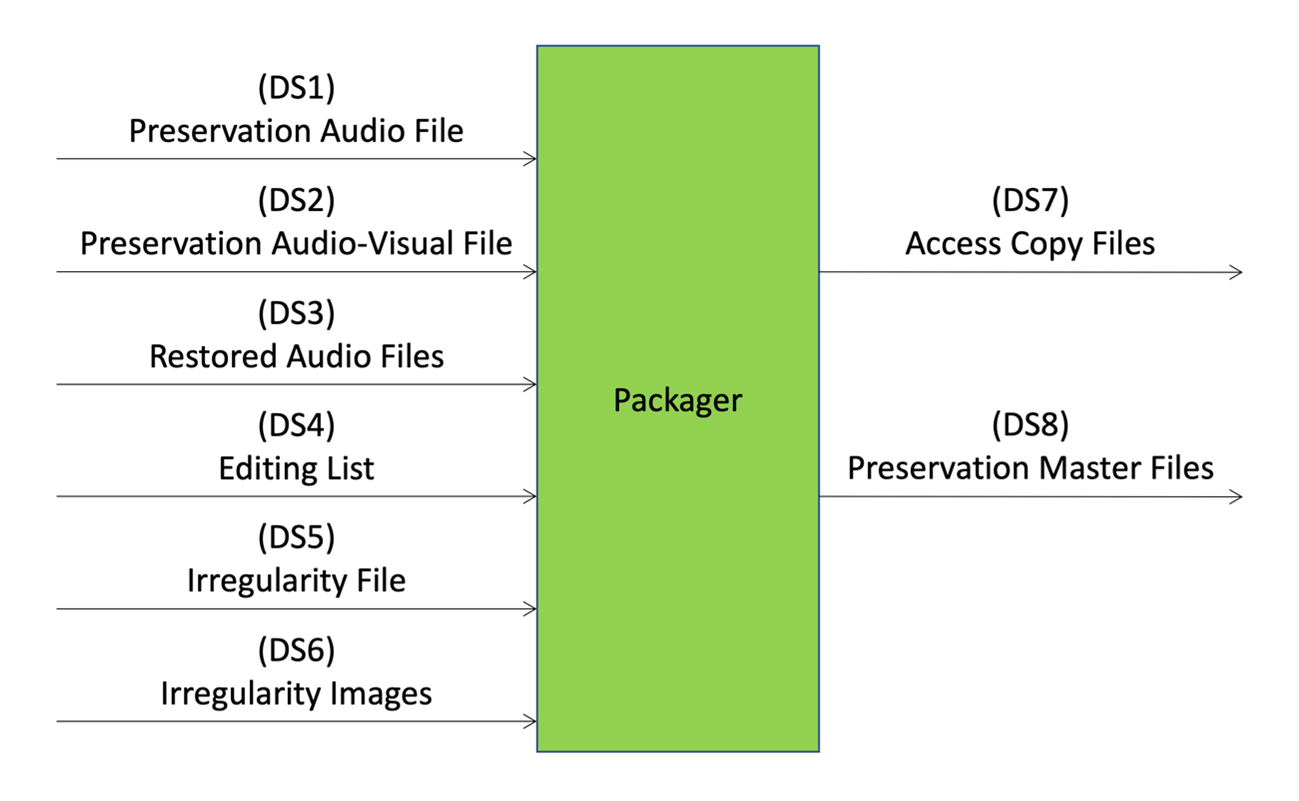
\includegraphics[width=0.9\textwidth]{packager.png}
    \caption{\ac{ARP} Packager}
    \label{fig:packager}
\end{figure}

% \begin{table}[h]
%     \centering
%     \begin{tabular}{|c|c|}
%         \hline
%         \textbf{Input data}             &   \textbf{Output Data}\\
%         \hline
%         Preservation Audio File         &   Access Copy Files\\
%         Preservation Audio-Visual File  &   Preservation Master Files\\
%         Restored Audio Files            &   \\
%         Editing List                    &   \\
%         Irregularity File               &   \\
%         Irregularity Images             &   \\
%         \hline
%     \end{tabular}
%     \caption{I/O di \ac{ARP} Packager}
%     \label{tab:packager-io}
% \end{table}

Il packager, come anticipato nella sottosezione \ref{ssec:mpai-cae-arp}, è l'ultimo \ac{AIM} ad essere eseguito e si occupa di raccogliere tutti i file elaborati e di restituire in uscita all'\ac{AIW} una cartella con la copia d'accesso dei file ed una con i file grezzi accompagnati da tutte le irregolarità trovate, vedi schema in figura \ref{fig:packager}.

Viene riportata la descrizione dei conformance tests da seguire, definita da MPAI, nella tabella \ref{tab:packager-valutazione}.\footnote{Estratta dalla versione WD 0.15.2 del documento MPAI Conformance Testing per \ac{CAE}.} 

\begin{table}[h]
    \centering
    \begin{tabular}{|p{0.2\textwidth}|p{0.8\textwidth}|}
        \hline
        \textbf{Means}   &   \textbf{Actions}\\
        \hline
        \textbf{Conformance Testing Dataset}    &
            DS1: n Preservation Audio Files.\newline
            DS2: n Preservation Audio-Visual Files related to DS1.\newline
            DS3: n Restored Audio Files arrays related to DS1 coming from Tape Audio Restoration.\newline
            DS4: n Editing Lists related to DS3 coming from Tape Audio Restoration.\newline
            DS5: n Irregularity Files related to DS1 coming from Tape Irregularity Classifier.\newline
            DS6: n Irregularity Images related to DS5 coming from Tape Irregularity Classifier.\newline
            DS7: n Access Copy Files.\newline
            DS8: n Preservation Master Files.\\
        \hline
        \textbf{Procedure}  &
            1.	Feed Packager under test with DS1, DS2, DS3, DS4, DS5 and DS6.\newline
            2.	Compare the output Access Copy Files with DS7.\newline
            3.	Compare the output Preservation Master Files with DS8.\\
        \hline
        \textbf{Evaluation} &
            For a given input tuple, verify that:\newline
                1.	The output Access Copy Files contain the Restored Audio Files, the Editing List, the Irregularity File and the set of Irregularity Images in a .zip file, and is therefore equal to DS7.\newline
                2.	The output Preservation Master Files contain the Preservation Audio File, the Preservation Audio-Visual File with the audio of the Preservation Audio File, the Irregularity File and the Irregularity Images, and is therefore equal to DS8.\newline
            An error on any of the output arrays will make the Packager under test not conformant.\\
        \hline
    \end{tabular}
    \caption{Test di conformità per \ac{ARP} Packager}
    \label{tab:packager-valutazione}
\end{table}


\subsection{Bug ed altri problemi pre-esistenti}    % moviepy vs ffmpeg (errori nel video e audio transcodifica in mp3), offset
Prima di dedicarsi alla scrittura dei test, si è verificata la corretta funzionalità del software.

Sono stati riscontrati dei problemi importanti relativi alla creazione del \textit{PreservationAudioVisualFile}

\begin{lstlisting}[language=Python, caption=Codice iniziale; creazione PreservationAudioVisualFile]
# Create Preservation Audio-Visual File with substituted audio
video_file = files_name + '.mov'
pvf_path = os.path.join(working_path, 'PreservationAudioVisualFile/', video_file)
try:
    audio = AudioFileClip(paf_path)
    video = VideoFileClip(pvf_path)
    # Open Irregularity File to get offset
    irregularity_file_json = open(
        os.path.join(temp_path, 'TapeIrregularityClassifier_IrregularityFileOutput2.json')
    )
    irregularity_file = json.load(irregularity_file_json)
    offset = irregularity_file['Offset']/1000
    if offset > 0:
        audio = audio.subclip(t_start=offset)
    else:
        video = video.subclip(t_start=offset)
    video = video.set_audio(audio)
    video.write_videofile(pmf_path + 'PreservationAudioVisualFile.mov', bitrate='3000k', codec='mpeg4')
    print("Preservation Audio-Visual File created")
except OSError:
    pprint(f"Preservation Audio-Visual File file '{pvf_path}' not found!", color=Color.RED)
    quit(os.EX_NOINPUT)
\end{lstlisting}

Il primo problema è relativo alla sincronizzazione del video con l'audio: l'audio deve essere anticipato se viene trovato un offset positivo, altrimenti deve essere anticipato il video.
Alle righe 12-16, si osserva che il comportamento non è quello richiesto, dato che a riga 16 l'offset ha valore negativo, allora \href{https://zulko.github.io/moviepy/}{MoviePy}, libreria utilizzata per eseguire editing video, farà iniziare la traccia a partire da $|offset|$ secondi prima del termine della clip.\footnote{Codice sorgente: \url{https://zulko.github.io/moviepy/_modules/moviepy/Clip.html#Clip.subclip}}    % TODO da verificare se vero

Il secondo problema è relativo alla non specifica nel codice della codifica audio che porta la libreria MoviePy a ricadere nel comportamento di default, ovvero generare un file con codifica MP3 (lossy) a \qty{44100}{\Hz} e ad avere di conseguenza, in questo caso, una transcodifica, il che non è ottimale per un software che ha come obiettivo la conservazione di documenti audio.

Il terzo problema invece è provocato dalla libreria \href{https://zulko.github.io/moviepy/}{MoviePy} che, per motivi sconosciuti e solo in alcuni casi, genera file corrotti nella traccia video, nello specifico che si bloccano dopo alcuni secondi.  % TODO verificare se c'entra con il problema di cui sopra.

Per risolvere questi due problemi si è scelto di sostituire MoviePy direttamente con \href{https://ffmpeg.org/}{FFmpeg}, ottenendo come risultato il seguente codice:
\begin{lstlisting}[language=Python, caption=Codice finale; creazione PreservationAudioVisualFile]
# Create Preservation Audio-Visual File with substituted audio
video_file = files_name + '.mov'
pvf_path = os.path.join(working_path, 'PreservationAudioVisualFile/', video_file)
try:
    # Open Irregularity File to get offset
    irregularity_file_json = open(
        os.path.join(temp_path, 'TapeIrregularityClassifier_IrregularityFileOutput2.json')
    )
    irregularity_file = json.load(irregularity_file_json)
    offset = irregularity_file['Offset']
    command_to_run = ['ffmpeg',
                      '-y', '-hide_banner', '-loglevel', 'error']
    # If offset is positive, the audio is anticipated, otherwise video is anticipated (through seek)
    if offset > 0:
        command_to_run = command_to_run + ['-i', pvf_path,
                                           '-ss', str(offset)+'ms', '-i', paf_path]
    else:
        command_to_run = command_to_run + ['-ss', str(offset * -1)+'ms', '-i', pvf_path,
                                           '-i', paf_path]
    command_to_run = command_to_run + ['-c:v', 'mpeg4', '-c:a', 'copy',
                                       '-map', '0:v', '-map', '1:a',
                                       '-b:v', '3M', '-maxrate', '4M', '-bufsize', '4M',
                                       pmf_path + 'PreservationAudioVisualFile.mov']
    subprocess.run(command_to_run)
    print("Preservation Audio-Visual File created")
except OSError:
    pprint(f"Preservation Audio-Visual File file '{pvf_path}' not found!", color=Color.RED)
    quit(os.EX_NOINPUT)
\end{lstlisting}


\subsection{Come verificare l'uguaglianza tra audio}  % fingerprinting con chromaprint, suo wrapper in python, open source software e mie contribuzioni, comunicare col mantainer
Per verificare l'uguaglianza fra tracce audio, inizialmente si è provato un confronto tramite le librerie \textit{hashlib} o \textit{filecmp}, ma entrambi i test non hanno avuto successo perchè in alcuni casi non è richiesto di verificare che il file sia lo stesso identico (stesso hash), ma piuttosto di controllare che il suono sia il medesimo\footnote{La differenza si osserva, per esempio, quando si hanno 2 file, uno scostato di qualche secondo rispetto all'altro, questo è ciò che accade nel caso in esame, quando si esegue la sincronizzazione audio/video.}.

La soluzione trovata si basa sulla libreria \href{https://acoustid.org/chromaprint}{chromaprint}\footnote{chromaprint è la libreria che è alla base del progetto AcoustID, utilizzato nel piuttosto famoso software \href{https://musicbrainz.org/}{MusicBrainz} (\href{https://picard.musicbrainz.org/}{Picard}) che serve a taggare le proprie tracce musicali.}, la quale permette di ricavare delle impronte digitali (\textit{fingerprint}) da delle tracce audio, in maniera da poi confrontarle tra loro per ottenere la loro somiglianza.    % TODO taggare va bene?

È stata utilizzata in particolare una libreria Python, la quale non è altro che un wrapper di AcoustID, chiamata \href{https://github.com/beetbox/pyacoustid}{pyacoustid} che aiuta lo sviluppatore Python esponendo direttamente le API di chromaprint ed un metodo per confrontare le impronte.

\begin{lstlisting}[language=Python, caption=Test di comparazione di due file audio tramite la loro impronta digitale]
AUDIO_THRESHOLD = 0.7
# [...]
input_fingerprint = acoustid.fingerprint_file(input_paf_path)
output_fingerprint = acoustid.fingerprint_file(output_paf_path)
assert acoustid.compare_fingerprints(input_fingerprint, output_fingerprint) > AUDIO_THRESHOLD, "PreservationAudioFile.wav is not the same as input"
\end{lstlisting}

Come si può leggere dal codice, è stata scelta come soglia di somiglianza il $70\%$, non è il $100\%$ perchè, ad esempio, nei casi in cui è stata effettuata la sincronizzazione audio/video l'audio non è esattamente uguale, inoltre dai vari test eseguiti sui dataset forniti, questo valore ha funzionato correttamente.

% TODO parlare di soglia scelta
Durante la scelta della soglia da adottare sono state eseguite diverse prove ed è interessante notare come




% TODO parlare di opensource blabla
% La libreria pyacoustid, nelle prime fasi di scrittura di 









\subsection{Come verificare l'uguaglianza tra video}  % ffmpeg e psnr
\subsection{Pulizia/reformat del codice della libreria} % principio DRY, docstrings, unit tests, compatiblità Windows ma esecuzione docker
\section{\acs{CAE}-\acs{ARP} audio analyser}
\subsection{Problemi pre-esistenti} % uso alias di pydantic ambiguo, typos, video analyser usa : invece di . e workaround, in Windows scipy.signal.correlate da overflow perche tipo di default per numpy è int32, test non funzionanti
\subsection{Come verificare che l'offset scelto è abbastanza vicino a quello reale} % formula fornita + ffprobe
\subsection{Come verificare che i file siano wav}   % RF64 ma in realtà va bene wav; libreria filetype, magic numbers, MIME
\subsection{Come verificare che la classificazione sia corretta}    % non necessario ma utile per capire che l'IA non da sempre stessi risultati, output utilizzati per gli altri test, recall, precision
\section{Parallelizzare o no? confronto di velocità} \label{sec:parallelizzazione}
\section{Libreria \texttt{mpai-cae-arp}}    % a cosa serve
\subsection{Bug: aggiornamento pydantic}    % che ha portato a dover aggiornare i moduli
\subsection{Bug: formatting sbagliato delle EditingList scritte su file}
\subsection{Bug: test di \texttt{AudioWave} a singolo canale non funzionante e fix di \texttt{get\_channel}}
\subsection{Aggiornamento delle librerie perchè cross-dependencies ora supportate (librosa, llvmlite, numpy)}
\subsection{Aggiornamento a Python 3.11} \label{ssec:py-311}

    %!TEX root = ../main.tex

\chapter{Conclusions and Future Works}
\label{chp:conclusions}

\begin{table}[ht]
    \centering
    \begin{tabular}{|l|l|}
    \hline
    \textbf{A} & \textbf{B} \\ \hline
    C          & D          \\ \hline
    E          & F          \\ \hline
    G          & H          \\ \hline
    \end{tabular}
    \caption{Table example \label{tab:table-name}}
\end{table}
    
    % Bibliography, appendix, acknowledges, etc...
    \backmatter
\end{document}